\frame{
    \frametitle{Current Set of Variables (Validated!)}
    \begin{center} \resizebox{\textheight}{!}{
        \begin{tabular}{ |l|l| }
        \hline
        \textbf {Histograms} & \textbf {Title} \\
        \hline
        jet\_count    &    BtagFexMT Number of Jets \\
        track\_count  &    BtagFexMT Number of Tracks \\
        vertex\_count &    BtagFexMT Number of Vertices \\
        jet\_pt       &  BtagFexMT Jet PT \\
        jet\_eta      &  BtagFexMT Jet Eta \\
        track\_Et     &    BtagFexMT Track Transverse Energy \\
        track\_eta    &    BtagFexMT Track Eta \\
        track\_phi    &    BtagFexMT Track Phi \\
        track\_d0     &    BtagFexMT Track D0 \\
        track\_d0err  &    BtagFexMT Track D0 Error \\
        track\_d0sig  &    BtagFexMT Track D0 Significance \\
        track\_z0     &    BtagFexMT Track Z0 \\
        track\_z0err  &    BtagFexMT Track Z0 Error \\
        track\_z0sig  &    BtagFexMT Track Z0 Significance \\
        \hline
    \end{tabular}
    } \end{center}
}

\frame{
    \frametitle{Current Set of Variables (Validated!)}
    (Fullsize images in backup...)
    \begin{columns}
        \begin{column}{0.6\textwidth}
            \resizebox{0.8\textheight}{!}{
                \begin{tabular}{ |l|l| }
                    \hline
                    \textbf {Histograms} & \textbf {Title} \\
                    \hline
                    jet\_count    &    BtagFexMT Number of Jets \\
                    track\_count  &    BtagFexMT Number of Tracks \\
                    vertex\_count &    BtagFexMT Number of Vertices \\
                    jet\_pt       &  BtagFexMT Jet PT \\
                    jet\_eta      &  BtagFexMT Jet Eta \\
                    track\_Et     &    BtagFexMT Track Transverse Energy \\
                    track\_eta    &    BtagFexMT Track Eta \\
                    track\_phi    &    BtagFexMT Track Phi \\
                    track\_d0     &    BtagFexMT Track D0 \\
                    track\_d0err  &    BtagFexMT Track D0 Error \\
                    track\_d0sig  &    BtagFexMT Track D0 Significance \\
                    track\_z0     &    BtagFexMT Track Z0 \\
                    track\_z0err  &    BtagFexMT Track Z0 Error \\
                    track\_z0sig  &    BtagFexMT Track Z0 Significance \\
                    \hline
                \end{tabular}
            }
        \end{column}
        \begin{column}{0.4\textwidth}
            \begin{figure}
                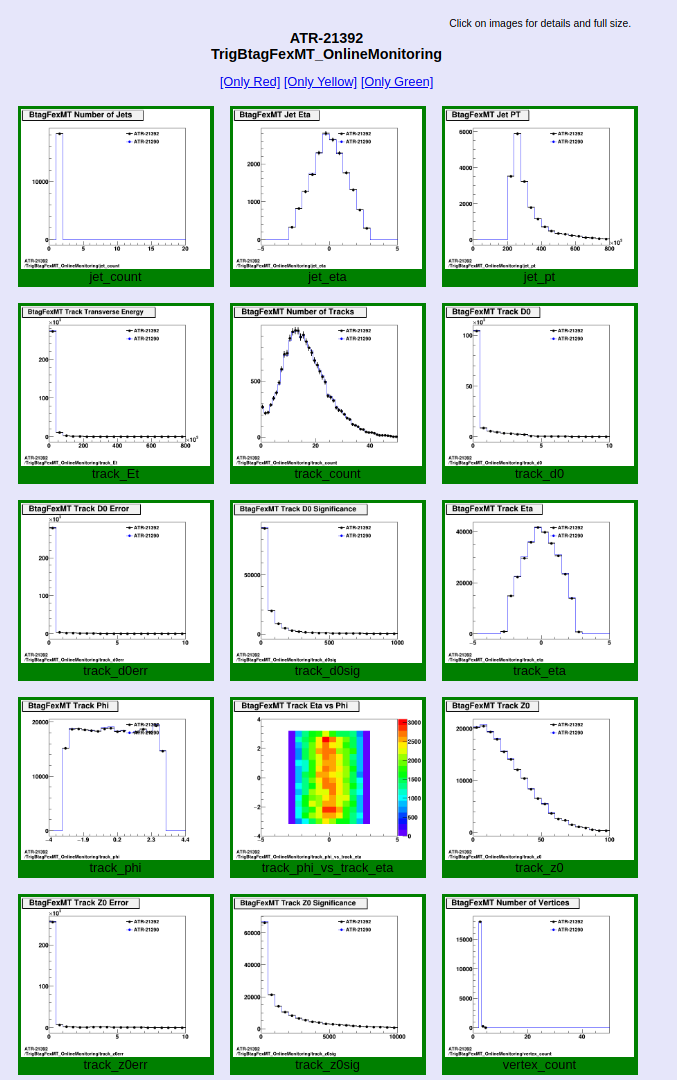
\includegraphics[height=0.8\textheight,keepaspectratio]{variables_signed_off}
            \end{figure}
        \end{column}
    \end{columns}
}
